\documentclass{beamer}
\usetheme{Szeged}
\usecolortheme{seahorse}
\usepackage{hyperref}
\usepackage[utf8]{inputenc}

\title{MathWorks Math Modelling Challenge 2019}
\author{Tristan Goodell, Nikki Weatherington, Jacob Holmes}
\institute[]{Arkansas School for Mathematics, Sciences, and the Arts}
\date{23 August 2019}

\begin{document}

\maketitle
 % To cite, use this: \footnote{Steward, Ian. Report: Americans Are Now More Likely To Die Of An Opioid Overdose Than On The Road. National Public Radio, 2019.} 
\begin{frame}{Introduction and Background}
    \begin{itemize}
    \item Our entry analyzed projected cigarette \& electronic cigarette use over the next 10 years, created a simulation of 300 high school seniors and predicts market share of Nicotine, Marijauna, alcohol, \& unprescribed opioids, and developed a comprehensive metric to calculate the impact of substance abuse.
        \item Data Sources:
        \begin{itemize}
            \item \href{https://m3challenge.siam.org/sites/default/files/uploads/high_school_vaping_data.xlsx}{High School Vaping Data}
            \item \href{https://m3challenge.siam.org/sites/default/files/uploads/NIH-DrugTrends-DataSheet\%20.xlsx}{NIH - DrugTrends - Data Sheet}
            \item \href{https://m3challenge.siam.org/sites/default/files/uploads/Figure_Adult\%20per\%20capita\%20cigarette\%20consumption\%20and\%20major\%20smoking\%20and\%20health\%20events_US_1900_2012.pdf}{Historical Cigarette Consumption}
        \end{itemize}
        \item Over the past 50 years, cigarette use has continued to decrease because of multiple efforts to improve legislature, broadcast health detriments, and help smokers become non-smokers.
        \item Over the past year, vaping use has increased by 50\%.  
    \end{itemize}
   
\end{frame}



\begin{frame}{Procedures}
    \begin{itemize}
        \item Darth Vapor
            \begin{itemize}
                \item We exported cigarette and e-cigarette usage data in 8th, 10th, \& 12th graders from 'NIH Drug Trends' for the years 2015 - 2018. Then, we performed a simple linear regression analysis. Finally, we extrapolated this model from 2015 to 2028. 
            \end{itemize}
        \item Above or Under the Influence
            \begin{itemize}
                \item For this simulation, we assumed that the drugs were not mutually exclusive and we ignored all external factors. We calculated the rates of Nicotine, Marijuana, Alcohol, and Unprescribed Opioids for seniors, and then performed a random simulation of 300 high school seniors. By using a combination of rand() and if() functions, we were able to develop a relatively accurate simulation. 
            \end{itemize}
    \end{itemize}
     \footnote{Steward, Ian. Report: Americans Are Now More Likely To Die Of An Opioid Overdose Than On The Road. National Public Radio, 2019.} 
\end{frame}

\begin{frame}{Analysis: Darth Vapor}
        \begin{itemize}
        \item As displayed in the graphs below, projected cigarette use in the next 10 years continues to decrease in 8th, 10th, \& 12th graders whilst vaping increases in 10th \& 12th graders. 
        \item In this projection, vaping rates in 8th graders do not change a statistically significant amount in the next 10 years. 
        \end{itemize}
    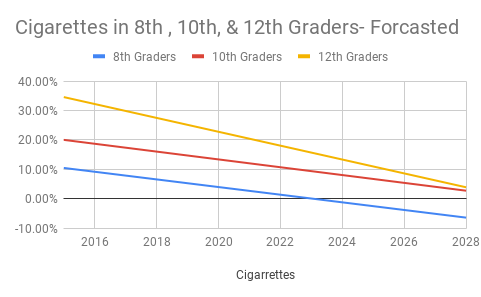
\includegraphics[scale=.35]{images/darthvapor-cigarettes.png}
    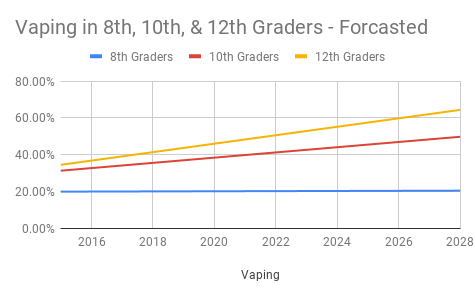
\includegraphics[scale=.35]{images/darthvapor-vaping.png}
    
    %You might choose to include a graph. Upload a .jpg or .png file and edit the code: \includegraphics[scale=1]{Name.jpg}
\end{frame}

\begin{frame}{Analysis: Above or Under the Influence?}
    \begin{itemize}
        \item In a simulation of 300 high school seniors, we observed the following:
        \begin{itemize}
            \item 156 seniors used Nicotine (52\%).
            \item 141 seniors used Marijuana (47\%). 
            \item 195 seniors used Alcohol (65\%). 
            \item 54 seniors used Unprescribed Opioids (18\%). 
        \end{itemize}
    \end{itemize}
\end{frame}

\begin{frame}{Analysis: Above or Under the Influence? - Cont.}
        \begin{center}
        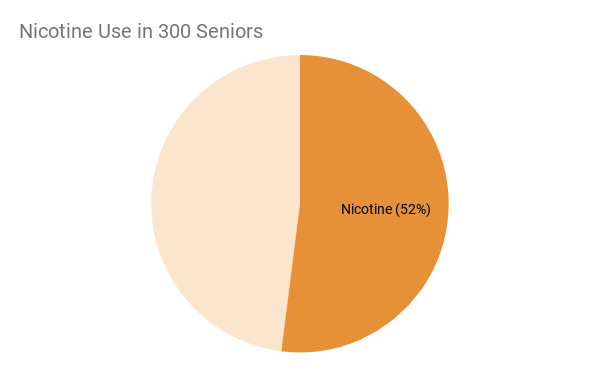
\includegraphics[scale=.25]{images/aboveunder-nicotine.png}
        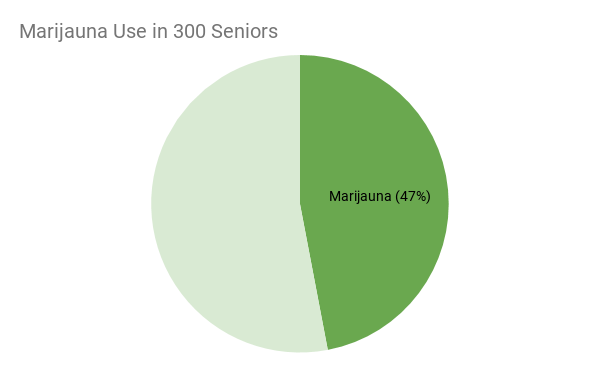
\includegraphics[scale=.25]{images/aboveunder-marijauna.png}
        
        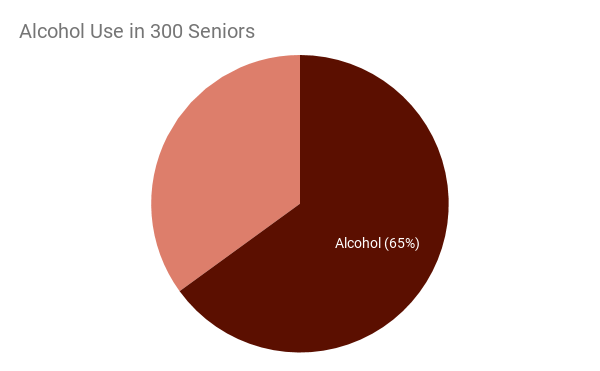
\includegraphics[scale=.25]{images/aboveunder-alcohol.png}
        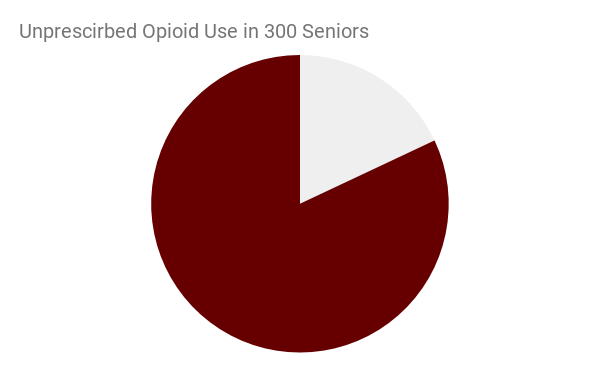
\includegraphics[scale=.25]{images/aboveunder-opioids.png}
    \end{center}
\end{frame}

\begin{frame}{Analysis: Ripples}
    \begin{itemize}
        \item We send out an annual survey to 8th - 12th graders. This survey takes into account drug usage in teens and average socioeconomic status of families in a specific district. 
        \item Various statistical tests can then be used to calculate the impact of the specified drug. 
    \end{itemize}
\end{frame}
%https://ecigarettereviewed.com/smoking-vs-vaping-cost-comparison

\begin{frame}{Conclusion}
        \begin{itemize}
        \item Vaping will increase over the next 10 years, and cigarette use will continue to decrease.
        \item Seniors in high school are over 50\% likely to use nicotine, marijuana, and/or alcohol.
        \item If we had more time to continue this project, we would like to apply multiple logistic functions to our data to better represent trend lines in Darth Vapor.
        \item Likewise, in Above or Under the Influence, we would like to find a better way to simulate the probabilities of seniors to use nicotine, marijuana, alcohol, and unprescribed opioids.
    \end{itemize}
\end{frame}

\end{document}
